\documentclass{beamer}
\usepackage[utf8]{inputenc}

\usepackage{utopia}
\setbeamerfont{caption}{series=\normalfont,size=\fontsize{8}{10}}

\usetheme{Madrid}
\usecolortheme{default}

\definecolor{RedCIMAT}{rgb}{0.44921875, 0.13671875, 0.234375}
\usecolortheme[named=RedCIMAT]{structure}

\setbeamertemplate{caption}[numbered]

\newcommand\Fontvi{\fontsize{10}{12.2}\selectfont}
\newcommand\FontEq{\fontsize{8}{12.2}\selectfont}

%------------------------------------------------------------
% Información de portada
\title[Detección de patologías pulmonares]{Detección de patologías pulmonares a través de modelos de aprendizaje profundo}
\subtitle{Tesis de Maestría}
\author[Oscar Esaú Peralta]{Oscar Esaú Peralta Rosales\\Director: Mariano JJ Rivera Meraz}
\institute[CIMAT]{Centro de Investigación en Matemáticas A.C.}
\date{Junio 2025}
\logo{
\includegraphics[height=0.7cm]{logo.jpg}}
%------------------------------------------------------------

\AtBeginSection[]
{
  \begin{frame}
    \frametitle{Tabla de Contenido}
    \tableofcontents[currentsection]
  \end{frame}
}

\begin{document}

\frame{\titlepage}

\begin{frame}
\frametitle{Tabla de Contenido}
\tableofcontents
\end{frame}

% --- INTRODUCCIÓN ---

% 01-Introduccion_Presentacion_Tesis.tex
% Diapositivas de la sección Introducción

\section{Introducción}

\begin{frame}
\frametitle{Contexto: COVID-19 y Salud Pública}
\begin{itemize}
    \item La pandemia de COVID-19 ha tenido un impacto sin precedentes:
    \begin{itemize}
        \item En salud y el bienestar de las personas
        \item En sistemas de salud a nivel mundial
    \end{itemize}
\end{itemize}

\begin{itemize}
    \item Alta demanda de atención médica
    \begin{itemize}
        \item Provocó saturación hospitalaria.
        \item Evidenció vulnerabilidad de los trabajadores de la salud.
    \end{itemize}
\end{itemize}
\end{frame}

\begin{frame}
\frametitle{Historia y Desafíos del COVID-19}
\begin{itemize}
    \item COVID-19 surge en 2019 en Wuhan, China, y es declarada pandemia en marzo de 2020.
    \item La ciencia y tecnología se convierten en herramientas clave para enfrentar estos retos.
    \item Urgencia de métodos que agilicen el diagnóstico y tratamiento de enfermedades pulmonares.
\end{itemize}
\end{frame}

\begin{frame}
\frametitle{Diagnóstico por Imágenes y Aprendizaje Automático}
\begin{itemize}
    \item El análisis de imágenes de rayos X y TC es fundamental para el diagnóstico de enfermedades pulmonares.
    \item Modelos de inteligencia artificial ayudan a identificar patologías y visualizar regiones de interés.
    \item Mejoran la precisión y rapidez del diagnóstico, optimizando recursos hospitalarios.
\end{itemize}
\end{frame}

\begin{frame}
\frametitle{Estado Actual de la Investigación}
\begin{itemize}
    \item A pesar de los avances, los métodos actuales enfrentan limitaciones importantes:
    \begin{itemize}
        \item Sesgos por bases de datos pequeñas o no normalizadas.
        \item Enfoques limitados a enfermedades específicas.
        \item Falta de regulación, validación y explicabilidad de los modelos.
    \end{itemize}
    \item Estas limitaciones dificultan su aplicación en entornos clínicos.
\end{itemize}
\end{frame}


% --- MOTIVACIÓN Y OBJETIVOS ---

% 02-Motivacion_Objetivos_Presentacion_Tesis.tex
% Diapositivas de la sección Motivación y Objetivos

\section{Motivación y Objetivos}

\begin{frame}
\frametitle{Motivación: Problema Relevante}
\begin{itemize}
    \item La detección de COVID-19 y otras patologías pulmonares mediante imágenes de rayos X es un reto relevante y desafiante.
    \item El diagnóstico temprano y preciso mejora el pronóstico y tratamiento de los pacientes.
    \item Reduce el riesgo de contagio y la carga sobre el sistema de salud.
\end{itemize}
\end{frame}

\begin{frame}
\frametitle{Oportunidades y Retos Específicos}
\begin{itemize}
    \item Disponibilidad de grandes volúmenes de datos y avances en arquitecturas de deep learning.
    \item Integración de datos heterogéneos y adaptación a escenarios clínicos reales.
    \item Necesidad de modelos interpretables y validados clínicamente.
    \item Desafío de implementar soluciones en entornos con recursos limitados.
\end{itemize}
\end{frame}

\begin{frame}
\frametitle{Propuesta de la Tesis}
\begin{itemize}
    \item Desarrollo de modelos de Deep Learning capaces de detectar múltiples patologías pulmonares, incluyendo COVID-19.
    \item Uso de imágenes de rayos X provenientes de diferentes fuentes y regiones.
    \item Comparación de modelos basados en Transformers y CNNs, ambos con técnicas de Transfer Learning.
    \item Evaluación mediante métricas de clasificación y visualización de regiones de interés.
\end{itemize}
\end{frame}

\begin{frame}
\frametitle{Ventajas del Modelo Propuesto}
\begin{itemize}
    \item \textbf{Diagnóstico múltiple y holístico}: detección simultánea de varias patologías.
    \item \textbf{Robustez ante variabilidad de datos}: diferentes calidades, resoluciones y contrastes.
    \item \textbf{Interpretabilidad}: generación de mapas de calor para validar las predicciones.
    \item \textbf{Herramienta de apoyo}: para el análisis exploratorio, no reemplazo del médico.
\end{itemize}
\end{frame}

\begin{frame}
\frametitle{Objetivos Específicos}
\begin{itemize}
    \item Desarrollar modelos de clasificación multiclase para 15 patologías pulmonares.
    \item Implementar y comparar arquitecturas basadas en Transformers y CNNs.
    \item Evaluar la robustez de los modelos ante diferentes fuentes de datos.
    \item Generar visualizaciones interpretables para validación clínica.
\end{itemize}
\end{frame}


% --- MARCO TEÓRICO ---

% 04-Marco_Teorico_Presentacion_Tesis.tex
% Diapositivas de la sección Marco Teórico

\section{Marco Teórico}

\begin{frame}
\frametitle{Redes Neuronales Convolucionales (CNN)}
\begin{itemize}
    \item Las CNN son la base del análisis de imágenes médicas.
    \item Permiten extraer características espaciales relevantes de las imágenes.
    \item Se utilizan ampliamente en tareas de clasificación, segmentación y detección.
\end{itemize}
\begin{figure}[ht!]
    \centering
    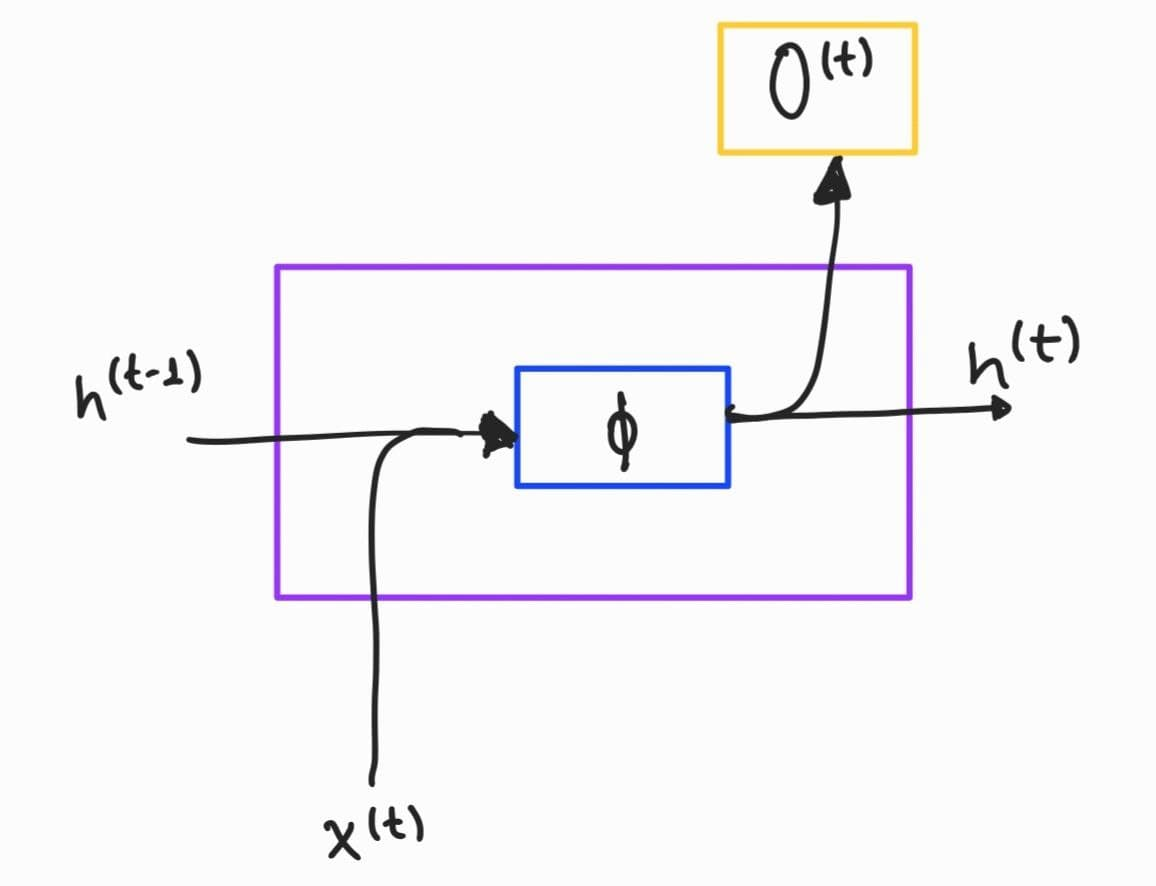
\includegraphics[width=0.5\textwidth]{../Chapters/2. Transformer/Figures/rnn/rnn_cell.jpg}
    \caption{Esquema de una red neuronal (referencial).}
\end{figure}
\end{frame}

\begin{frame}
\frametitle{ResNet50: Arquitectura Residual}
\begin{itemize}
    \item ResNet50 es una arquitectura profunda con 50 capas y conexiones residuales.
    \item Facilita el entrenamiento de redes muy profundas evitando el problema del desvanecimiento del gradiente.
    \item En esta tesis, ResNet50 se emplea como backbone para la extracción de características en imágenes de rayos X.
\end{itemize}
\end{frame}

\begin{frame}
\frametitle{Redes Neuronales Recurrentes (RNN)}
\begin{itemize}
    \item Las RNN procesan secuencias de datos, manteniendo información temporal.
    \item Son útiles para tareas donde el contexto previo es importante.
    \item Existen variantes como LSTM y GRU que mejoran la capacidad de memoria.
\end{itemize}
\begin{figure}[ht!]
    \centering
    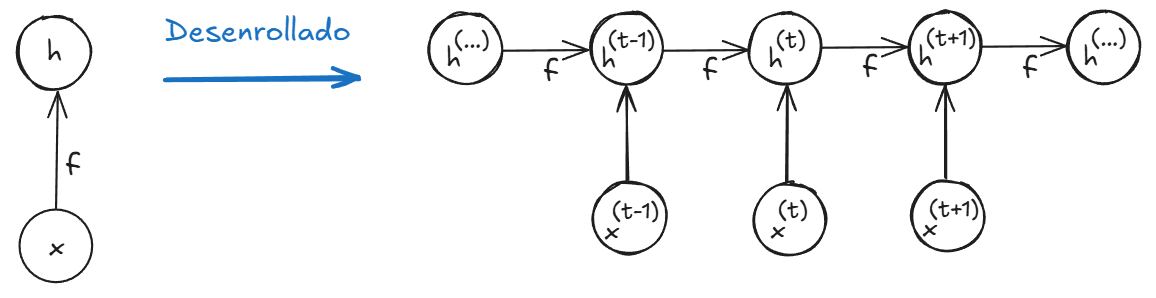
\includegraphics[width=0.7\textwidth]{../Chapters/2. Transformer/Figures/rnn/rnn_cgraph.png}
    \caption{Grafo computacional de una RNN desenrollada.}
\end{figure}
\end{frame}

\begin{frame}
\frametitle{Mecanismos de Atención y Transformers}
\begin{itemize}
    \item Los mecanismos de atención permiten al modelo enfocarse en partes relevantes de la entrada.
    \item Los Transformers revolucionaron el procesamiento de secuencias al permitir el procesamiento paralelo y el uso de atención múltiple (Multi-Head Attention).
    \item Vision Transformer (ViT) aplica estos conceptos a imágenes.
\end{itemize}
\end{frame}

\begin{frame}
\frametitle{Resumen del Marco Teórico}
\begin{itemize}
    \item Se combinan arquitecturas convolucionales (ResNet50) y modelos basados en atención (Transformers) para la detección de patologías pulmonares.
    \item El uso de Transfer Learning y Fine-Tuning permite adaptar modelos preentrenados a imágenes médicas.
    \item Estas técnicas mejoran la precisión y la interpretabilidad en el diagnóstico asistido por IA.
\end{itemize}
\end{frame}


% --- METODOLOGÍA ---

% 05-Metodologia_Presentacion_Tesis.tex
% Diapositivas de la sección Metodología

\section{Metodología}

\begin{frame}
\frametitle{Flujo General de la Metodología}
\begin{itemize}
    \item Desarrollo de modelos de aprendizaje profundo para la detección de 15 patologías pulmonares en rayos X.
    \item Dos enfoques principales: ResNet50 (CNN) y Vision Transformer (ViT).
    \item Proceso estructurado: preprocesamiento, entrenamiento, evaluación y extensión a nuevas patologías.
\end{itemize}
\end{frame}

\begin{frame}
\frametitle{Bases de Datos y Composición}
\begin{itemize}
    \item Uso del dataset ChestX-ray14 (112,120 imágenes, 30,805 pacientes, 14 patologías).
    \item Extensión con imágenes de COVID-19 y saludables.
    \item Re-etiquetado de datos usando modelos automáticos para mejorar la calidad de las etiquetas.
\end{itemize}
\end{frame}

\begin{frame}
\frametitle{Preprocesamiento de Imágenes}
\begin{itemize}
    \item Redimensionamiento a $1024 \times 1024$ y $384 \times 384$ píxeles según el modelo.
    \item Normalización y estandarización de intensidades.
    \item Data augmentation: rotaciones, traslaciones, escalados y flips para robustez.
\end{itemize}
\end{frame}

\begin{frame}
\frametitle{Entrenamiento: Transfer Learning y Fine-Tuning}
\begin{itemize}
    \item ResNet50 y ViT preentrenados en ImageNet.
    \item Tres etapas: (1) Transfer learning (cambio de la capa de salida), (2) Fine-tuning de las últimas capas, (3) Full-tuning de toda la red.
    \item Permite adaptar modelos generales a tareas médicas específicas con menos datos.
\end{itemize}
\end{frame}

\begin{frame}
\frametitle{Arquitectura de los Modelos}
\begin{columns}
\column{0.5\textwidth}
\textbf{ResNet50}
\begin{itemize}
    \item Red convolucional profunda con conexiones residuales.
    \item Extrae características espaciales de las radiografías.
\end{itemize}
\column{0.5\textwidth}
\textbf{Vision Transformer (ViT)}
\begin{itemize}
    \item Divide la imagen en parches y los procesa como una secuencia.
    \item Utiliza mecanismos de atención para capturar relaciones globales.
\end{itemize}
\end{columns}
\begin{figure}[ht!]
    \centering
    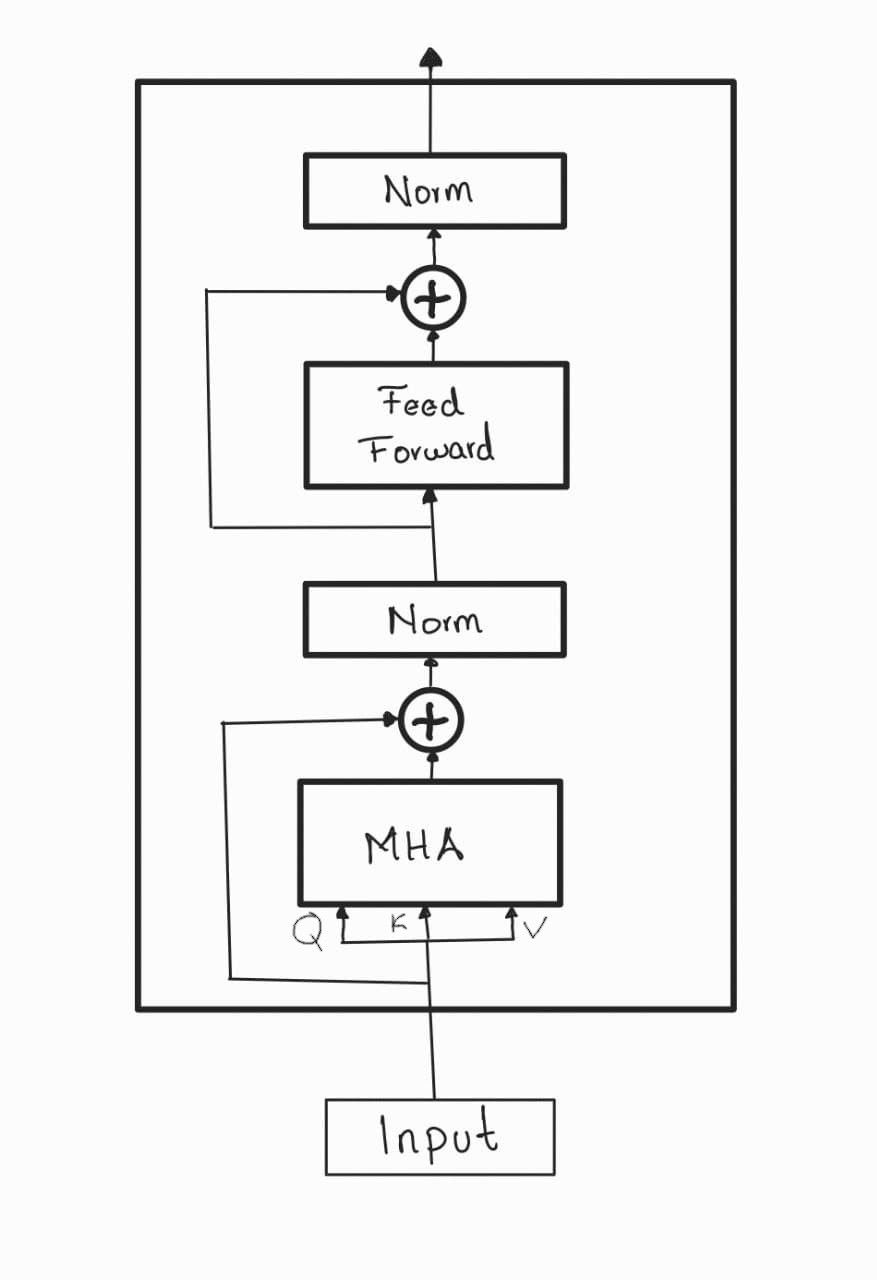
\includegraphics[width=0.7\textwidth]{../Chapters/2. Transformer/Figures/transformer/encoder.jpg}
    \caption{Esquema de codificador Transformer (ViT).}
\end{figure}
\end{frame}

\begin{frame}
\frametitle{Evaluación y Métricas}
\begin{itemize}
    \item División de datos en entrenamiento, validación y prueba.
    \item Métricas: AUC, precisión, recall, F1-score y matriz de confusión.
    \item Visualización de resultados: mapas de calor y curvas ROC.
\end{itemize}
\begin{figure}[ht!]
    \centering
    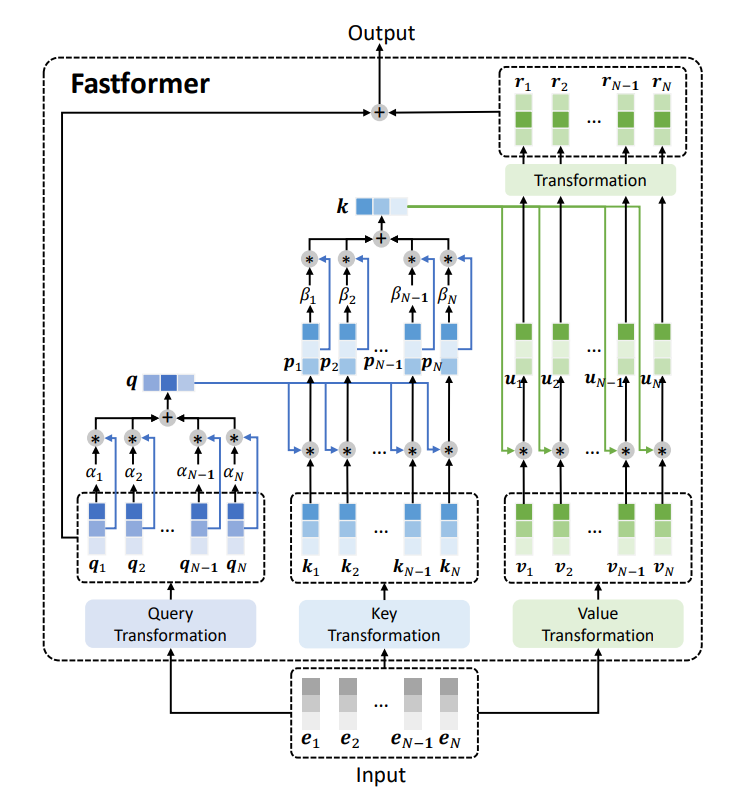
\includegraphics[width=0.7\textwidth]{../Chapters/2. Transformer/Figures/transformer/fastformer.png}
    \caption{Ejemplo de visualización de atención en modelos tipo Transformer.}
\end{figure}
\end{frame}

\begin{frame}
\frametitle{Extensión y Generalización}
\begin{itemize}
    \item El modelo puede ser extendido fácilmente a nuevas patologías (ejemplo: tuberculosis).
    \item El proceso de re-etiquetado y entrenamiento permite adaptar el sistema a diferentes escenarios clínicos.
    \item Resultados competitivos frente al estado del arte en todas las patologías evaluadas.
\end{itemize}
\end{frame}


% --- RESULTADOS ---

% 06-Resultados_Presentacion_Tesis.tex
% Diapositivas de la sección Resultados

\section{Resultados}

\begin{frame}
\frametitle{Evaluación de los Modelos}
\begin{itemize}
    \item Se evaluaron dos modelos principales: ResNet50 (CNN) y Vision Transformer (ViT).
    \item Ambos modelos fueron entrenados para detectar 15 patologías pulmonares, incluyendo COVID-19.
    \item Se utilizaron métricas como AUC-ROC, AUC-PR, F1-Score y Accuracy.
\end{itemize}
\end{frame}

\begin{frame}
\frametitle{Métricas de Evaluación}
\begin{itemize}
    \item \textbf{AUC-ROC}: Área bajo la curva ROC, mide la capacidad de discriminación del modelo.
    \item \textbf{AUC-PR}: Área bajo la curva Precisión-Recall, útil en clases desbalanceadas.
    \item \textbf{F1-Score}: Media armónica entre precisión y recall.
    \item \textbf{Accuracy}: Proporción de clasificaciones correctas.
\end{itemize}
\end{frame}

\begin{frame}
\frametitle{Comparativa de Resultados Globales}
\begin{itemize}
    \item Ambos modelos muestran resultados competitivos en la detección de patologías pulmonares.
    \item El modelo ViT destaca en la detección de COVID-19 y otras patologías complejas.
    \item ResNet50 mantiene un rendimiento robusto y eficiente en la mayoría de las clases.
\end{itemize}
\end{frame}

\begin{frame}
\frametitle{Resultados por Patología (AUC-ROC)}
\begin{figure}[ht!]
    \centering
    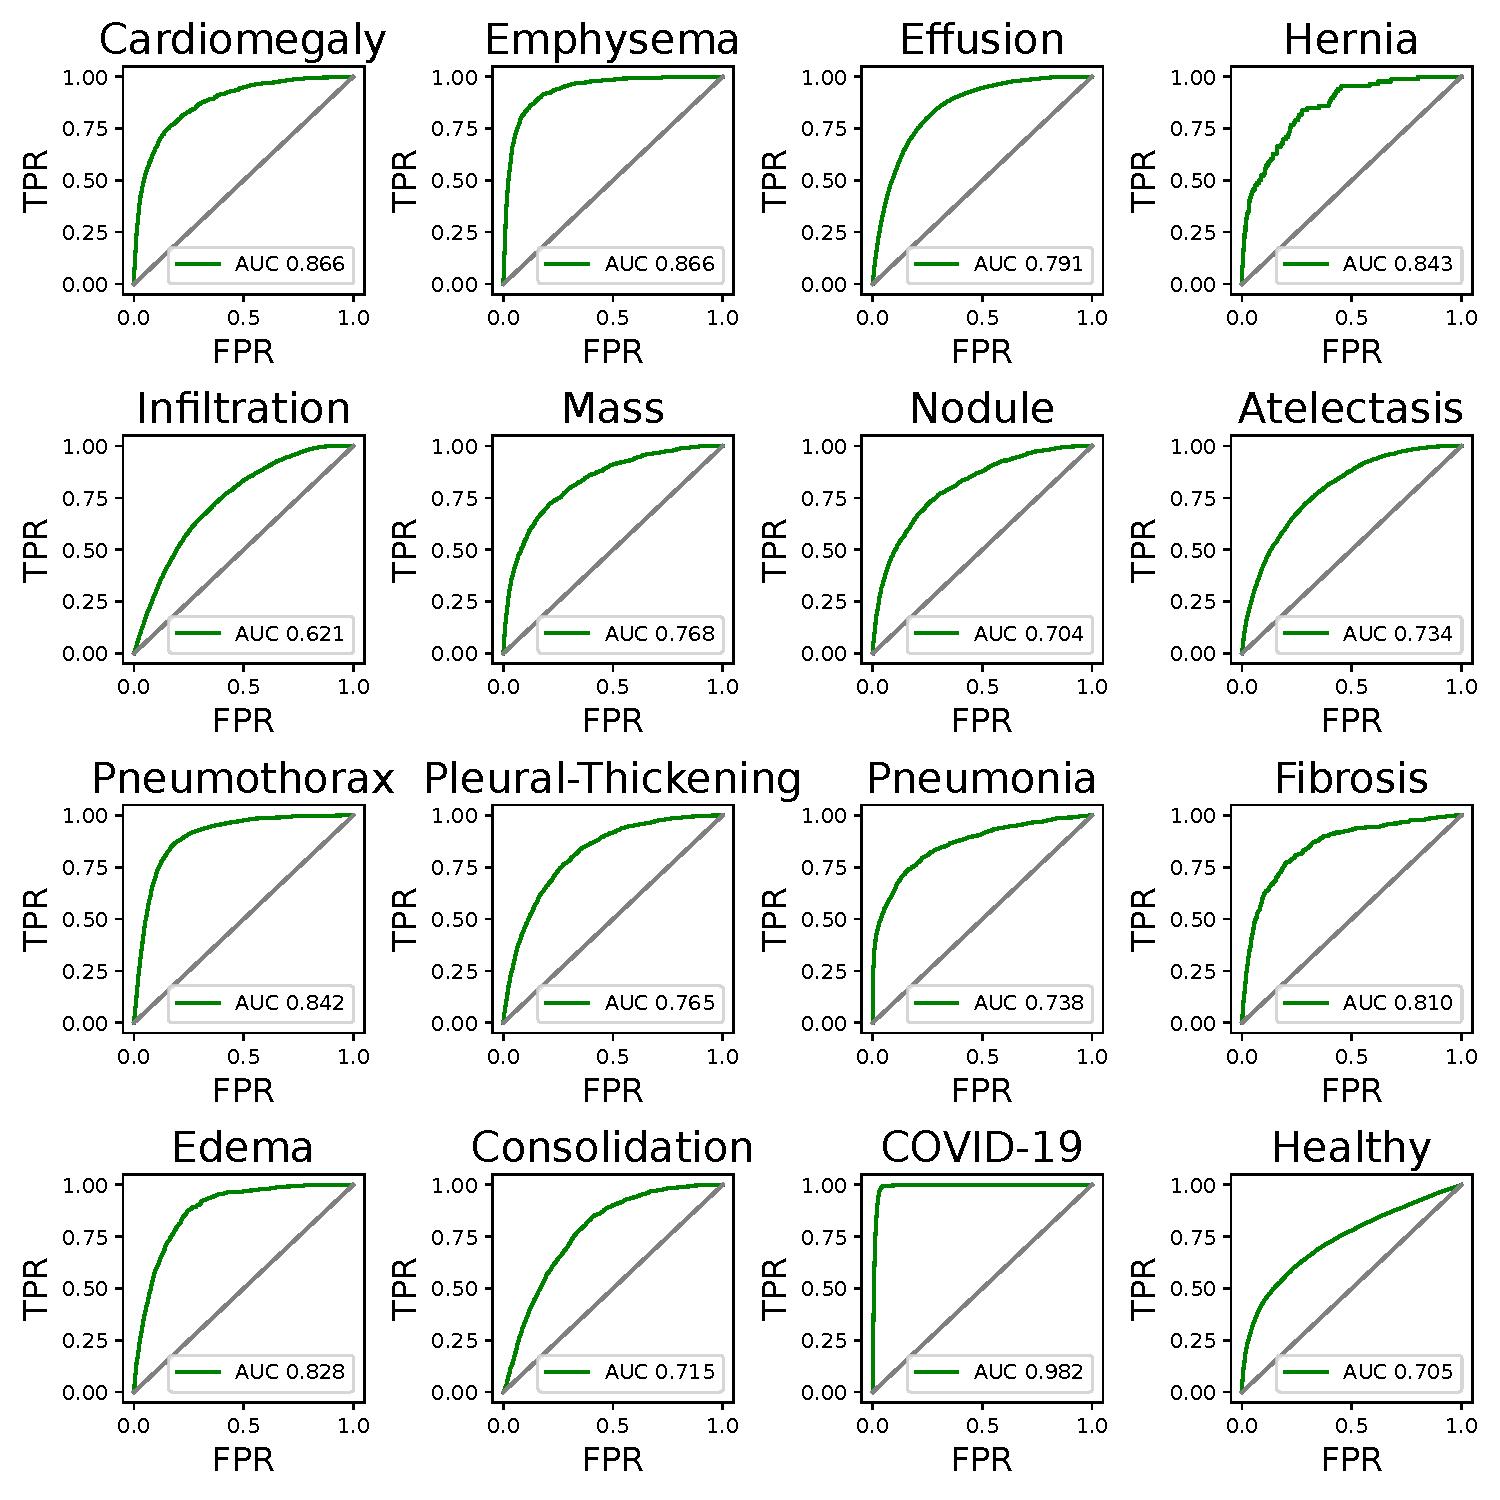
\includegraphics[width=0.9\textwidth]{../Chapters/4. ViT-Lung/images/ROC_AUC_ViT.pdf}
    \caption{Curvas ROC para las principales patologías detectadas por el modelo ViT.}
\end{figure}
\end{frame}

\begin{frame}
\frametitle{Visualización de la Atención del Modelo}
\begin{figure}[ht!]
    \centering
    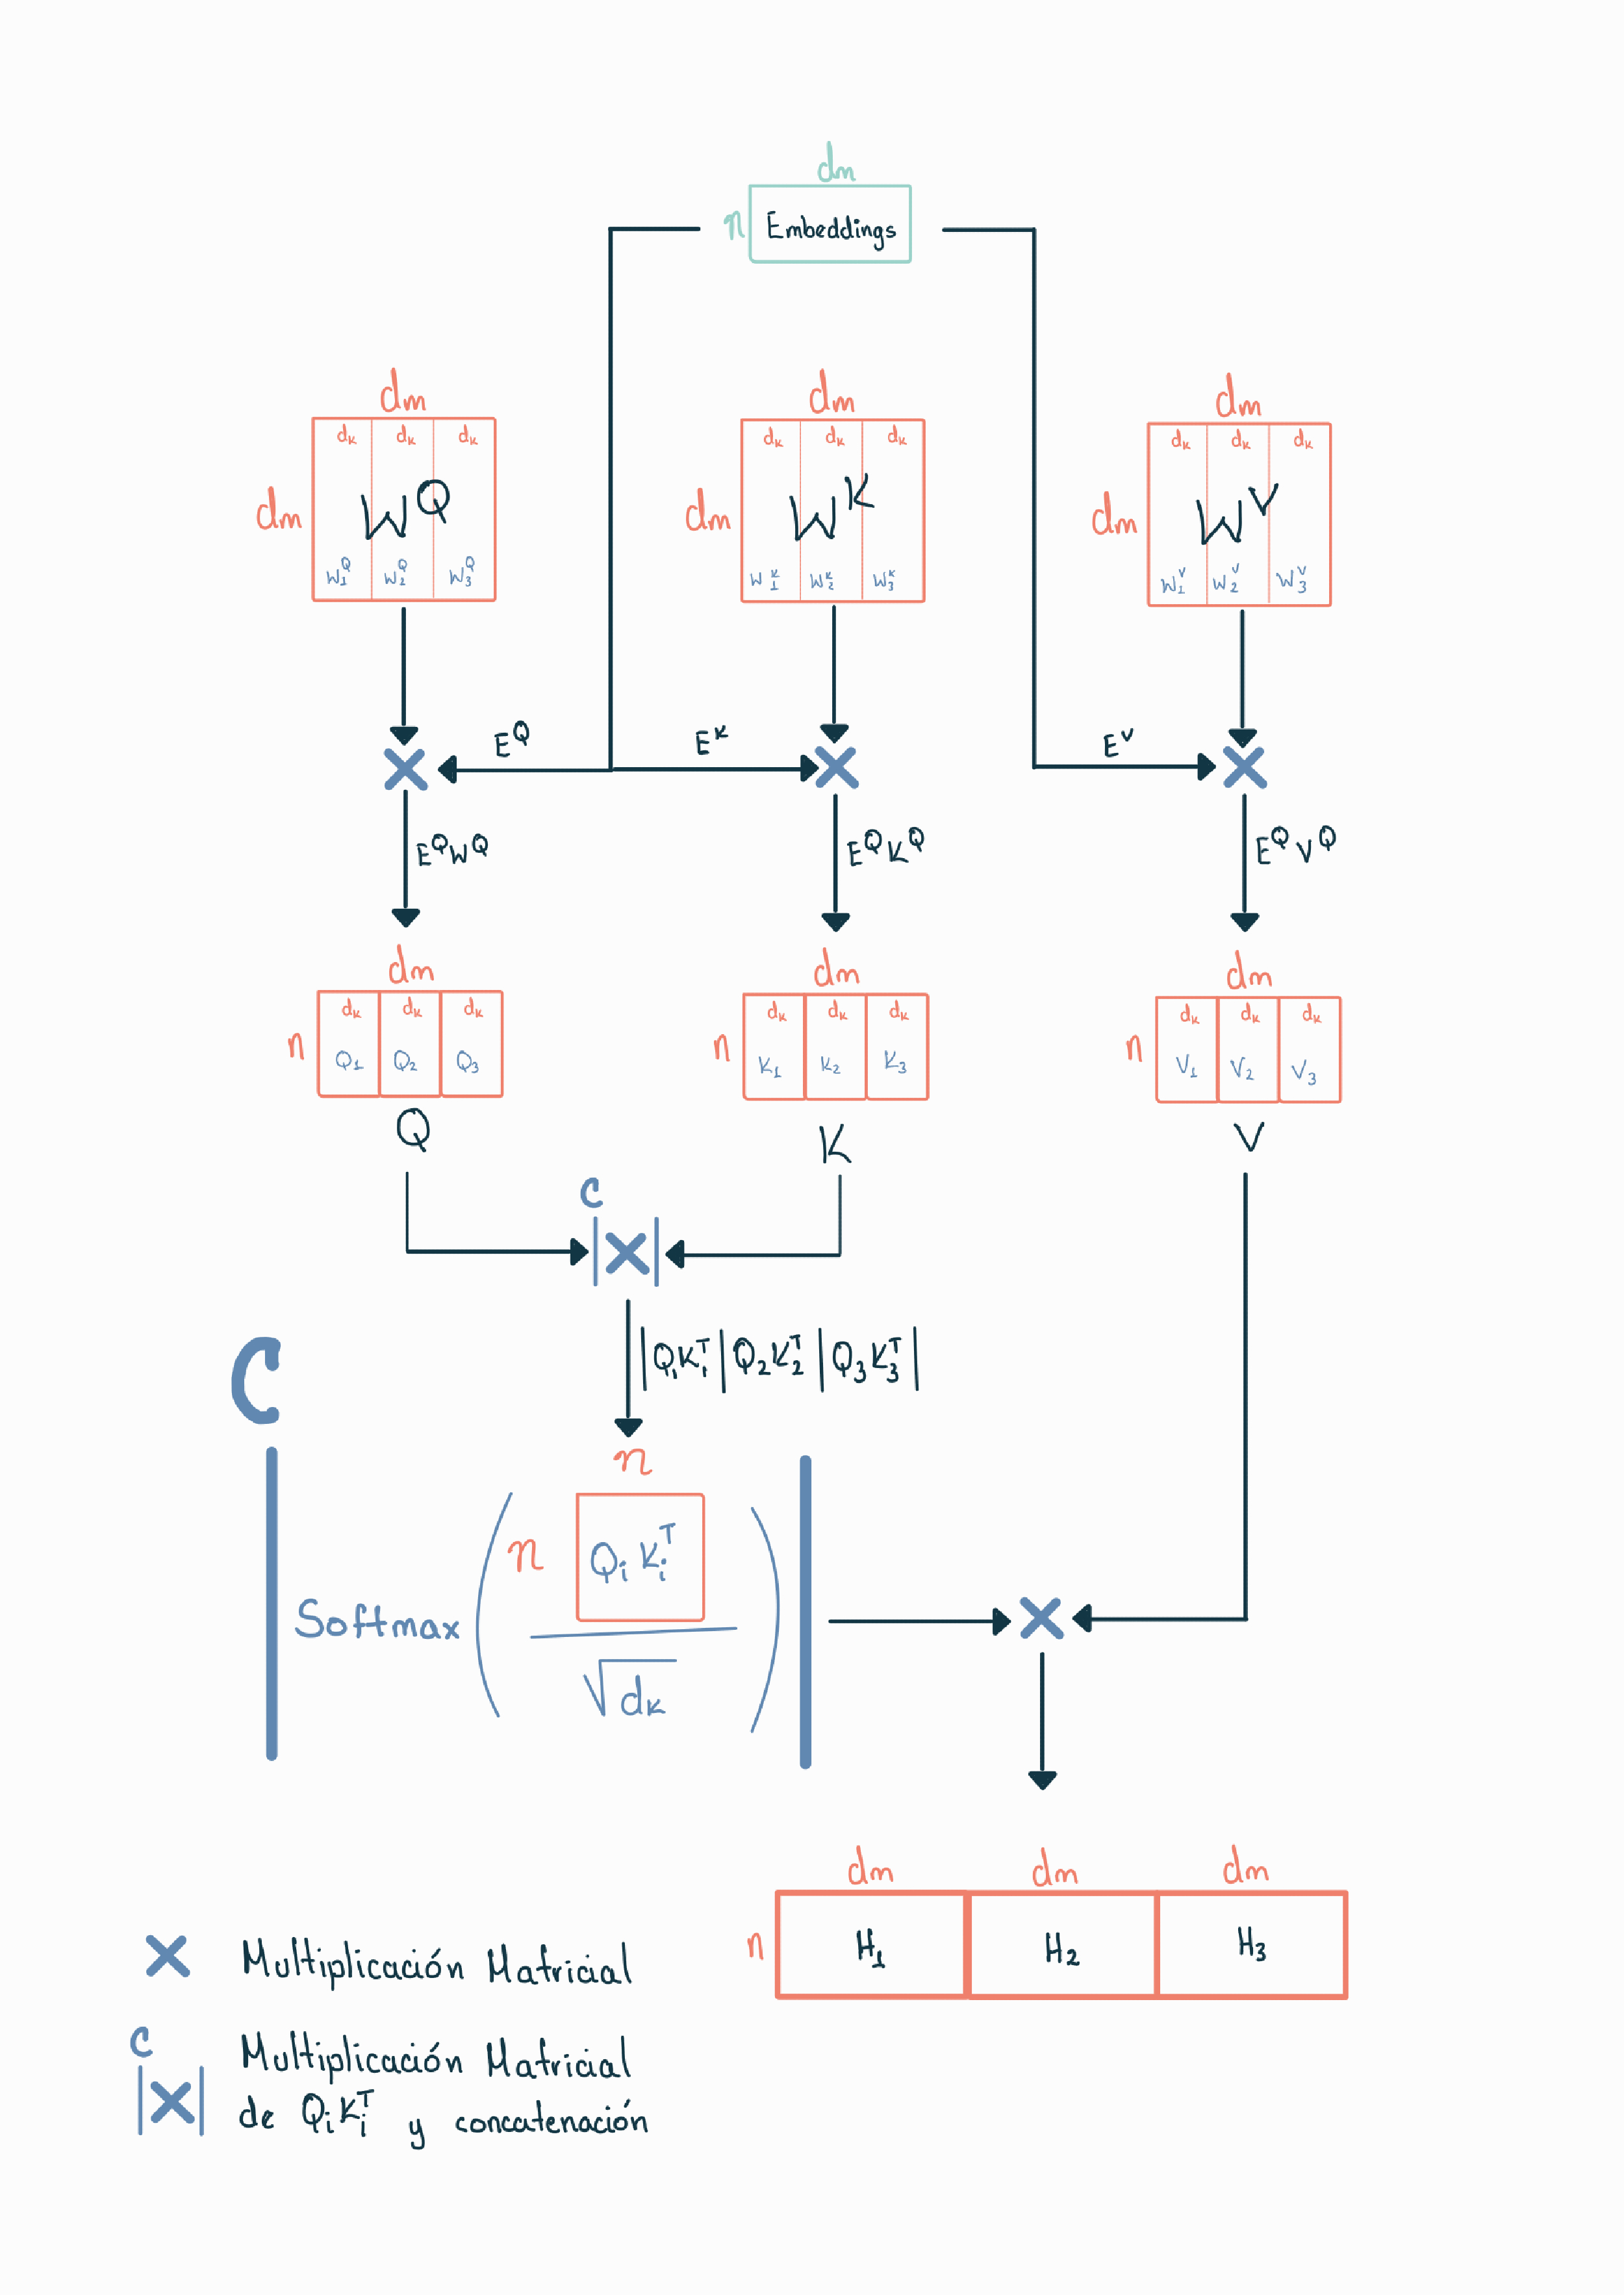
\includegraphics[width=0.7\textwidth]{../Chapters/4. ViT-Lung/images/cabezas_vit.jpg}
    \caption{Visualización de las cabezas de atención en el modelo ViT.}
\end{figure}
\end{frame}

\begin{frame}
\frametitle{Resumen de Resultados}
\begin{itemize}
    \item Ambos modelos superan o igualan el estado del arte en la mayoría de las patologías.
    \item El modelo ViT es especialmente competitivo en la detección de COVID-19.
    \item La arquitectura propuesta permite extender fácilmente la detección a nuevas patologías.
\end{itemize}
\end{frame}


% --- CONCLUSIONES Y TRABAJO FUTURO ---

% 07-Conclusiones_TrabajoFuturo_Presentacion_Tesis.tex
% Diapositivas de la sección Conclusiones y Trabajo Futuro

\section{Conclusiones y Trabajo Futuro}

\begin{frame}
\frametitle{Conclusiones}
\begin{itemize}
    \item Se desarrollaron dos modelos de aprendizaje profundo para el diagnóstico de 15 patologías pulmonares, incluyendo COVID-19, a partir de imágenes de rayos X.
    \item Ambos modelos muestran rendimiento comparable o superior al estado del arte, especialmente en la detección de COVID-19.
    \item El uso de Transfer Learning y arquitecturas como ResNet50 y Vision Transformer permite extender fácilmente la detección a nuevas patologías.
\end{itemize}
\end{frame}

\begin{frame}
\frametitle{Ventajas y Limitaciones}
\begin{itemize}
    \item Modelos robustos y precisos, útiles como herramienta de apoyo para radiólogos.
    \item Facilidad de extensión a otras enfermedades pulmonares, como la tuberculosis.
    \item Limitaciones: calidad y representatividad de los datos, falta de validación clínica, y recursos computacionales limitados.
\end{itemize}
\end{frame}

\begin{frame}
\frametitle{Trabajo Futuro}
\begin{itemize}
    \item Mejorar la calidad y diversidad de las bases de datos de imágenes.
    \item Explorar nuevas arquitecturas y técnicas de aprendizaje profundo.
    \item Incorporar otras modalidades de imagen, como tomografía computarizada.
    \item Desarrollar herramientas visuales y mapas de calor para facilitar el diagnóstico.
    \item Validación clínica y regulación de los modelos para su uso real.
\end{itemize}
\end{frame}


% --- AGRADECIMIENTOS ---

% 08-Agradecimientos_Presentacion_Tesis.tex
% Diapositivas de la sección Agradecimientos

\section{Agradecimientos}

\begin{frame}
\frametitle{Agradecimientos}
\begin{itemize}
    \item A mi director de tesis, Dr. Mariano J. J. Rivera Meraz, por su invaluable orientación, paciencia y apoyo constante.
    \item A mi familia, especialmente a mis padres Gabina Rosales Garnica y Alejandro Peralta Sosa, y a mis hermanos Itandehui y Ovidio Alejandro, por su amor y apoyo incondicional.
    \item A María del Rosario Jiménez Cabrera, por su amor, apoyo y motivación constante.
    \item A mis compañeros y amigos, en especial a Daniel Martínez Tovar, Pablo Antonio Stack Sánchez y Marco Antonio Esquivel Basaldua, por su ayuda y amistad.
    \item Al Centro de Investigación en Matemáticas (CIMAT), profesores y personal administrativo, por el entorno y recursos brindados.
    \item A todos los participantes, organizaciones y comunidades que facilitaron el acceso a los datos y colaboraron en la investigación.
    \item Y a todas las personas que, de una u otra manera, contribuyeron al desarrollo de esta tesis.
\end{itemize}
\end{frame}


\begin{frame}
\begin{center}
    Gracias por su atención.
\end{center}
\end{frame}

\end{document}
